\subsection{Kategorisering af KOL-patienter} \label{sec:kategorisering}
Førend KOL-patienter kan benytte app'en til træning skal en individuel kategorisering af patienten forekomme. Dette er nødvendigt for således at sikre patienter får en træning tilpasset til deres niveau. 
Hertil placeres patienter i ABCD-kategorisering, der er beskrevet i \autoref{sec:klassifikation}. Af \autoref{fig:Kate} ses aktivitetsdiagrammet for denne kategorisering.

\begin{figure} [H]
\centering
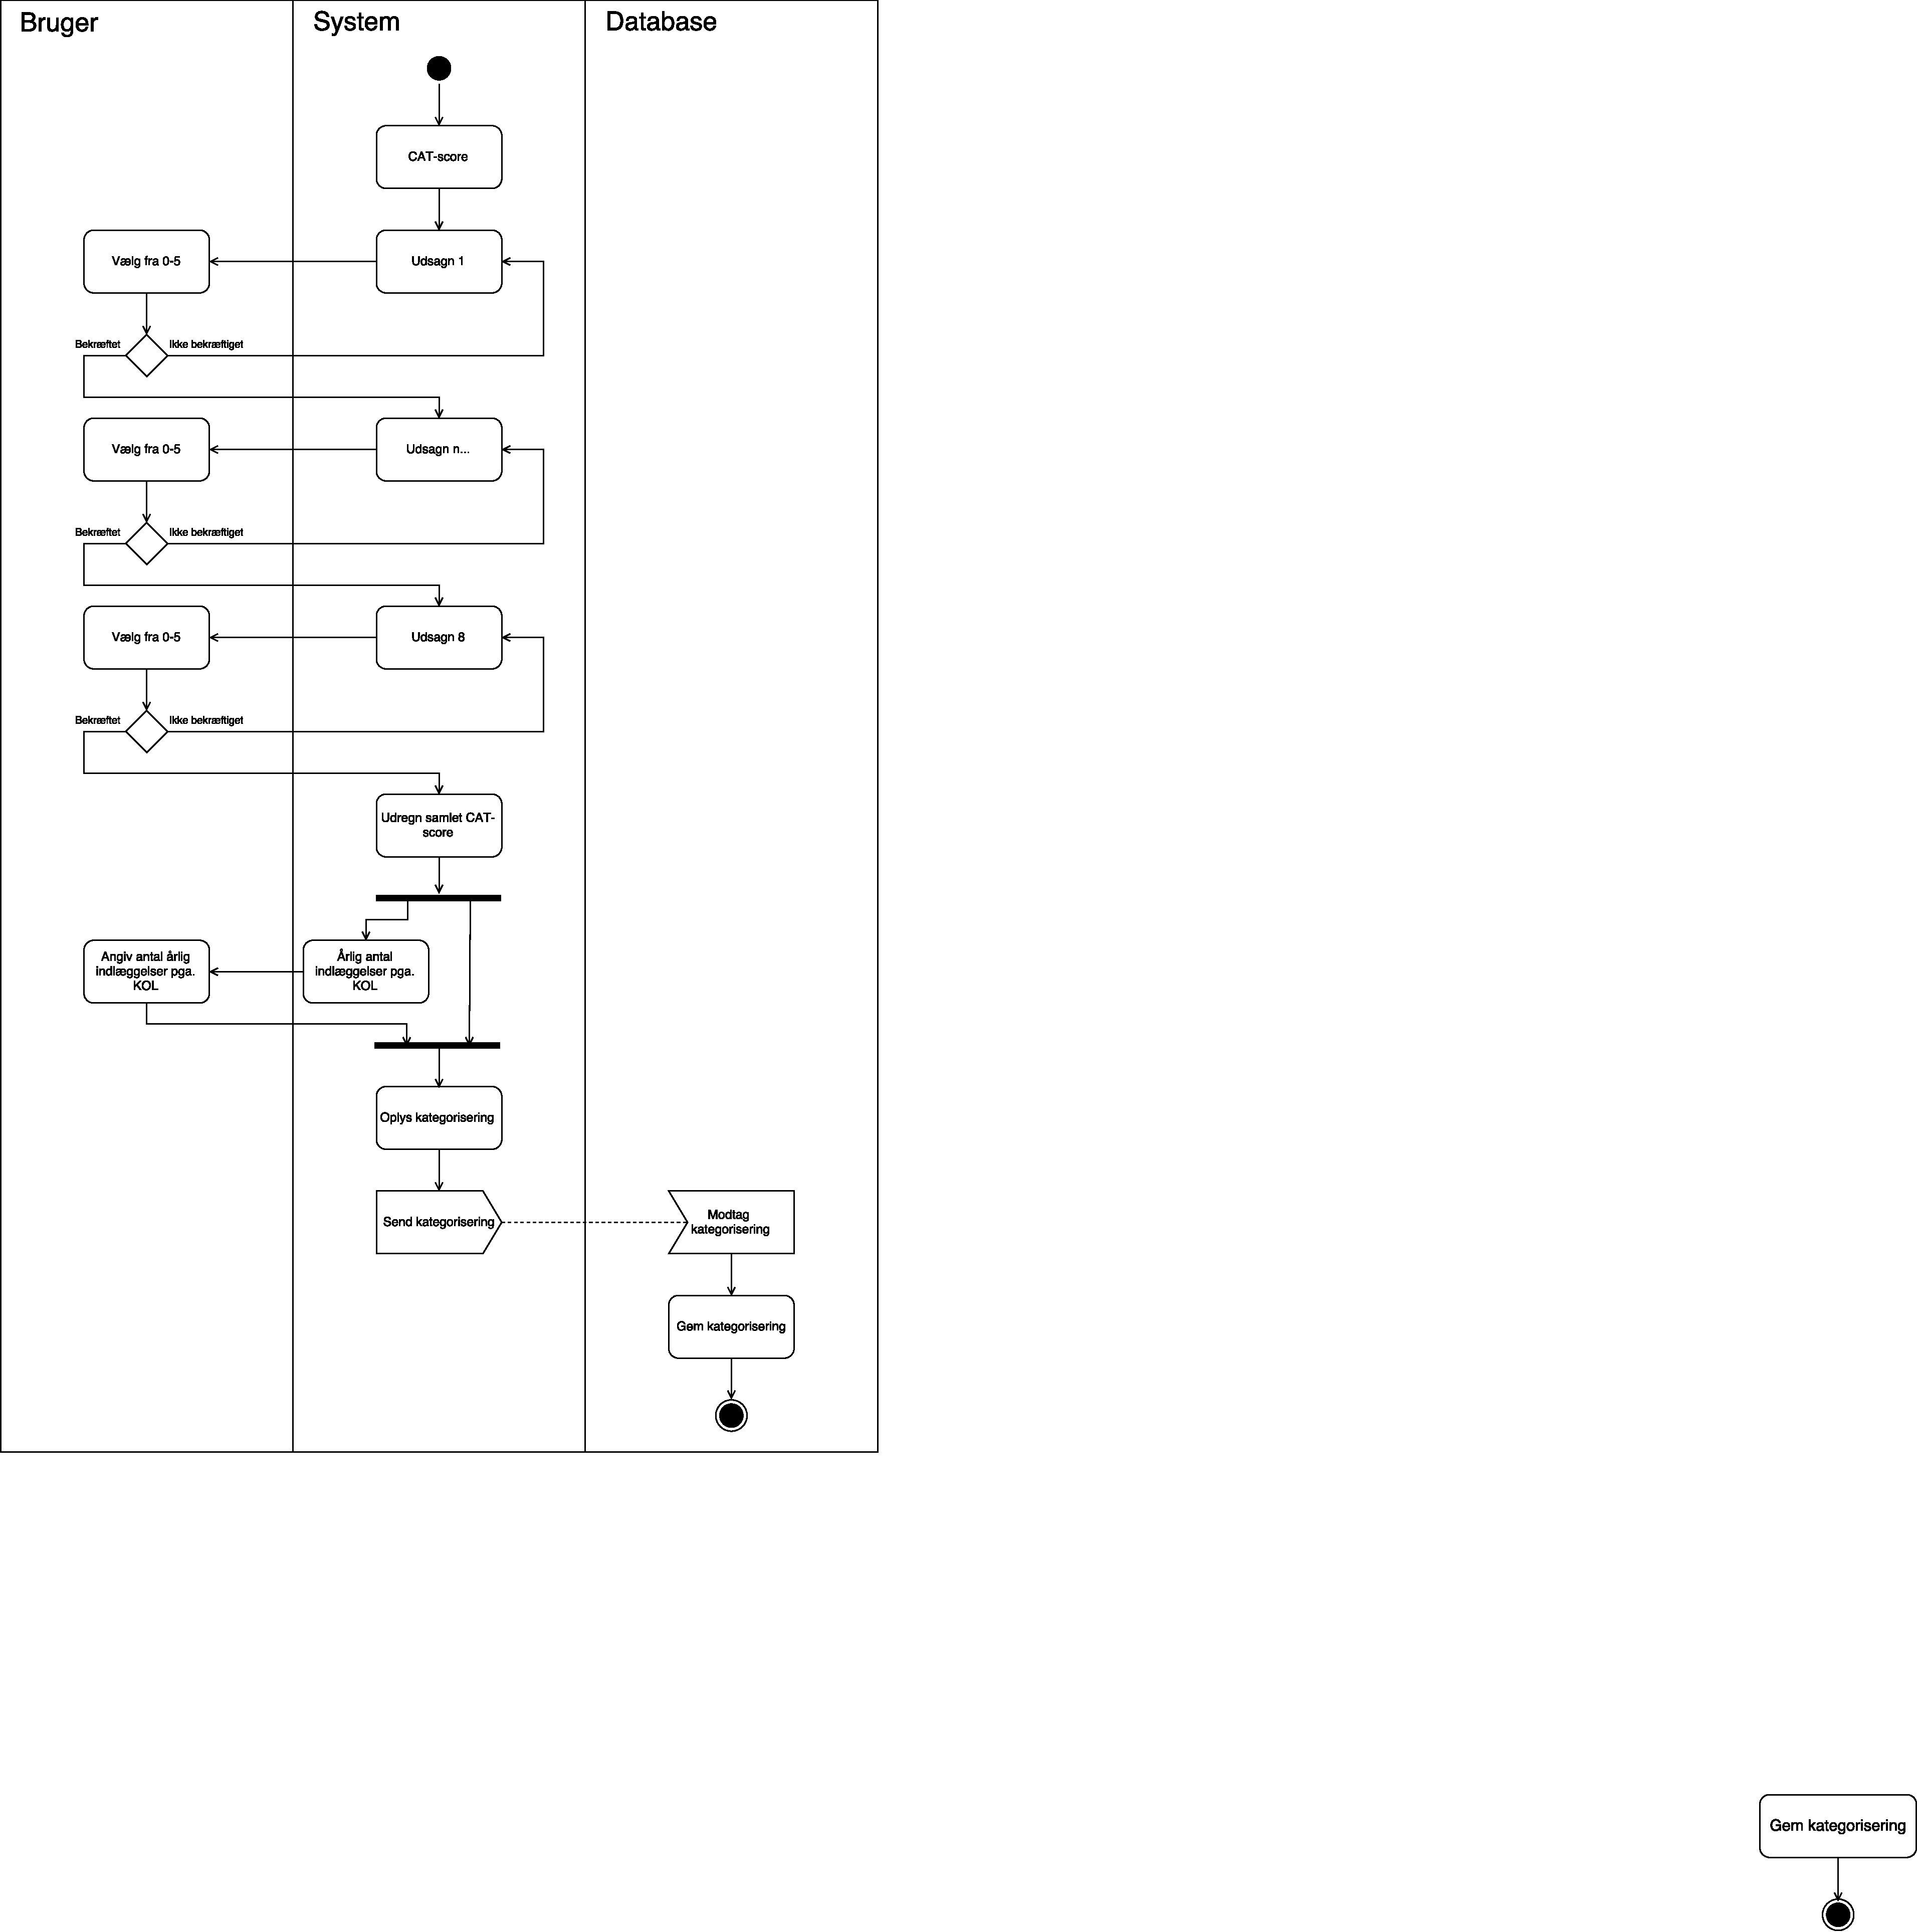
\includegraphics[width=0.65\textwidth]{figures/aktivitetsdiagram/Kategorisering}
\caption{Aktivitetsdiagram for kategorisering af KOL-patienter.}
\label{fig:Kate}
\end{figure}

\noindent
KOL-patienter kategoriseres første gang de logger ind på app'en. Derudover kan kategoriseringen redigeres, jf. \autoref{sec:redigering}, i tilfælde af, at KOL-patienters tilstand ændres.
Brugeren stilles otte udsagn, hvorved de vurderer deres tilstand fra 0 til 5. Tilstanden skal herefter bekræftiges af brugeren, hvis det ikke bekræftes stilles det førhenværende udsagn igen. På baggrund af vurderingen fra udsagnene udregnes den samlede CAT-score. Herefter skal brugeren angive antal indlæggelser forårsaget af KOL inden for det seneste år som værende ingen eller én til flere indlæggelser. Ud fra den samlede CAT-score samt de årlige indlæggelser oplyses ABCD-kategoriseringen af patienten. 